%%%%%%%%%%%%%%%%%%%%%%%%%%%%%%%%%%%%%%%%%
% Beamer Presentation
% LaTeX Template
% Version 1.0 (10/11/12)
%
% This template has been downloaded from:
% http://www.LaTeXTemplates.com
%
% License:
% CC BY-NC-SA 3.0 (http://creativecommons.org/licenses/by-nc-sa/3.0/)
%
%%%%%%%%%%%%%%%%%%%%%%%%%%%%%%%%%%%%%%%%%

%----------------------------------------------------------------------------------------
%	PACKAGES AND THEMES
%----------------------------------------------------------------------------------------

\documentclass{beamer}

\mode<presentation> {

% The Beamer class comes with a number of default slide themes
% which change the colors and layouts of slides. Below this is a list
% of all the themes, uncomment each in turn to see what they look like.

%\usetheme{default}
%\usetheme{AnnArbor}
%\usetheme{Antibes}
%\usetheme{Bergen}
%\usetheme{Berkeley}
%\usetheme{Berlin}
%\usetheme{Boadilla}
%\usetheme{CambridgeUS}
%\usetheme{Copenhagen}
%\usetheme{Darmstadt}
%\usetheme{Dresden}
%\usetheme{Frankfurt}
%\usetheme{Goettingen}
%\usetheme{Hannover}
%\usetheme{Ilmenau}
%\usetheme{JuanLesPins}
%\usetheme{Luebeck}
\usetheme{Madrid}
%\usetheme{Malmoe}
%\usetheme{Marburg}
%\usetheme{Montpellier}
%\usetheme{PaloAlto}
%\usetheme{Pittsburgh}
%\usetheme{Rochester}
%\usetheme{Singapore}
%\usetheme{Szeged}
%\usetheme{Warsaw}

% As well as themes, the Beamer class has a number of color themes
% for any slide theme. Uncomment each of these in turn to see how it
% changes the colors of your current slide theme.

%\usecolortheme{albatross}
%\usecolortheme{beaver}
%\usecolortheme{beetle}
%\usecolortheme{crane}
%\usecolortheme{dolphin}
%\usecolortheme{dove}
%\usecolortheme{fly}
%\usecolortheme{lily}
%\usecolortheme{orchid}
%\usecolortheme{rose}
%\usecolortheme{seagull}
%\usecolortheme{seahorse}
%\usecolortheme{whale}
%\usecolortheme{wolverine}

%\setbeamertemplate{footline} % To remove the footer line in all slides uncomment this line
%\setbeamertemplate{footline}[page number] % To replace the footer line in all slides with a simple slide count uncomment this line

%\setbeamertemplate{navigation symbols}{} % To remove the navigation symbols from the bottom of all slides uncomment this line
}

\usepackage{graphicx} % Allows including images
\usepackage{booktabs} % Allows the use of \toprule, \midrule and \bottomrule in tables

%----------------------------------------------------------------------------------------
%	TITLE PAGE
%----------------------------------------------------------------------------------------

\title[Newton Bases and PDEs]{Kernel Newton Bases for solving PDEs} % The short title appears at the bottom of every slide, the full title is only on the title page

\author{Tim McCollam, Palmer Lao} % Your name
\institute[IIT, CU] % Your institution as it will appear on the bottom of every slide, may be shorthand to save space
{
Illinois Institute of Technology, Clarkson University \\ % Your institution for the title page
\medskip
\textit{tmccolla@hawk.iit.edu, laopa@clarkson.edu} % Your email address
}
\date{\today} % Date, can be changed to a custom date

\begin{document}

\begin{frame}
\titlepage % Print the title page as the first slide
\end{frame}

%----------------------------------------------------------------------------------------
%	PRESENTATION SLIDES
%----------------------------------------------------------------------------------------


\begin{frame}
\frametitle{Motivation}
\begin{itemize}
\item A famous example in 1-D of an ill-conditioned interpolation matrix is the Vandermonde matrix
\item Instead of monomials, we can use a different basis to get a better-conditioned matrix
\item Examples include the Lagrange basis and the Newton basis
\end{itemize}
\end{frame}

\begin{frame}
\frametitle{Multivariate Interpolation}
\begin{itemize}
\item In the multivariate case, we need to use data-dependent basis elements (kernels) because of Curtis-Mairhuber
\item Interpolation matrices formed using the translated kernel basis are often ill-conditioned, esp. when smoothness increases
\item In 2009, Müller and Schaback published a paper applying the idea of Newton bases to kernel interpolation
\item The condition number of the interpolation matrix is much better
\end{itemize}
\end{frame}

\begin{frame}
\frametitle{Newton Basis Refresher}
\begin{itemize}
\item Each basis element is of the form $v_j = \prod_{i=0}^{j-1}(x-x_i)$
\item The $j$th basis element evaluated at $x_i$ is 0 whenever $i < j$. This results in a lower triangular interpolation matrix
\item The matrix is better conditioned as well as easier to solve numerically, although the coefficients can be found using divided differences instead
\end{itemize}
\end{frame}

\begin{frame}
\frametitle{Kernel Newton Bases}
\begin{itemize}
\item Without Newton Bases, to interpolate a function $u$, we choose to represent it as the linear combination of translated kernels: $u(x) \approx \sum_{j=0}^n c_j K(x, x_j)$
\item We would then need to solve a linear system of equations for $c_j$, $j=0,...,n$, which usually involves inverting $\mathbf{K} = (K(x_i,x_j))_{i,j=0}^n$
\end{itemize}
\centering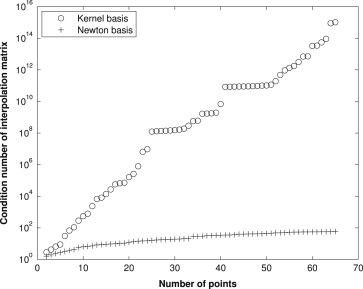
\includegraphics[scale=0.6]{ill_cond}

\end{frame}

\begin{frame}
\frametitle{Kernel Newton Bases (cont.)}
\begin{itemize}
\item Since $\mathbf{K}$ is often ill-conditioned, we instead need functions $v_0, ..., v_n$ such that span$\{ v_0, ... v_j \} = $ span$\{K(\cdot, x_0), ..., K(\cdot, x_j)\}$ for $j=0,...,n$. %v_0 ... v_n is the Newton Bases
\item Copying an idea from the polynomial version of the Newton form, we also require that $v_j(x_j) = 1$ and $v_j(x_i) = 0$ when $i = 0, ..., j-1$.
\end{itemize}
\end{frame}

\begin{frame}
\frametitle{Collocation for solving PDEs numerically}
\begin{itemize}
\item Collocation is closely related to interpolation, and the collocation matrix may also suffer from conditioning issues
\item Suppose we wish to solve $Lu = f$, where $L$ is a known linear operator. Again, assume $u(x) \approx \sum_{j=0}^n c_j K(x, x_j)$
\item Then we need to solve  $(LK(x_i, x_j))_{i,j=0}^n \mathbf{c} = \mathbf{f} = (f(x_i))_{i=0}^n$ for $\mathbf{c}$ 
\item We hope to figure out how to differentiate the Newton basis elements to improve conditioning in the collocation matrix.
\end{itemize}
\end{frame}

\begin{frame}
\frametitle{Another way of solving PDEs numerically}
\begin{itemize}
\item From our expansion of $u$ as a combination of our basis functions, we have the following system: $\mathbf{K}\mathbf{c} = \mathbf{u}$
\item Instead of forcing the solution to satisfy constraints at collocation points, create a pointwise approximation to the linear operator using a matrix.
\item We need a matrix $D$ such that $D \mathbf{u} \approx \left( Lu(x_i) \right)_{i=0}^n \approx D \mathbf{K} \mathbf{c} $.
\item Choose $D = LK(x_i, x_j) _{i,j=0}^n \mathbf{K}^{-1}$, then $D\mathbf{u} \approx D\mathbf{K}\mathbf{c} = \left( Lu(x_i) \right)_{i=0}^n \mathbf{c} = \mathbf{f}$. 
\item We need to invert $D$ to get values of $u$
\end{itemize}
\end{frame}

%------------------------------------------------

\begin{frame}
\Huge{\centerline{Thanks!}}
\end{frame}

%----------------------------------------------------------------------------------------

\end{document} 